% This file was created by tikzplotlib v0.9.8.
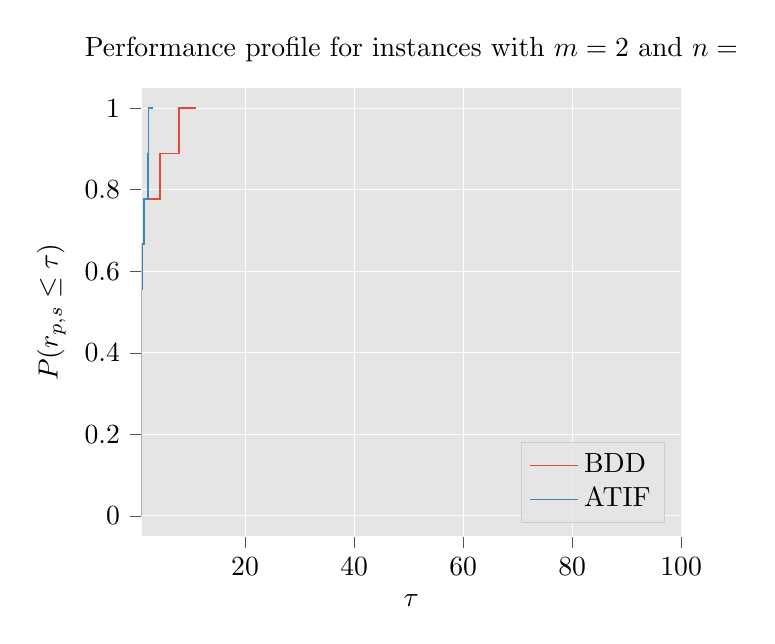
\begin{tikzpicture}

\definecolor{color0}{rgb}{0.886274509803922,0.290196078431373,0.2}
\definecolor{color1}{rgb}{0.203921568627451,0.541176470588235,0.741176470588235}

\begin{axis}[
axis background/.style={fill=white!89.8039215686275!black},
axis line style={white},
legend cell align={left},
legend style={
  fill opacity=0.8,
  draw opacity=1,
  text opacity=1,
  at={(0.97,0.03)},
  anchor=south east,
  draw=white!80!black,
  fill=white!89.8039215686275!black
},
tick align=outside,
tick pos=left,
title={Performance profile for instances with \(\displaystyle m = 2\) and \(\displaystyle n = \)},
x grid style={white},
xlabel={\(\displaystyle \tau\)},
xmajorgrids,
xmin=1, xmax=100,
xtick style={color=white!33.3333333333333!black},
y grid style={white},
ylabel={\(\displaystyle P(r_{p,s} \leq \tau)\)},
ymajorgrids,
ymin=-0.05, ymax=1.05,
ytick style={color=white!33.3333333333333!black}
]
\addplot [semithick, color0, const plot mark right]
table {%
1 0
1 0.111111111111111
1 0.222222222222222
1 0.333333333333333
1 0.444444444444444
1.10255680892608 0.555555555555556
1.50886419791667 0.666666666666667
4.45043880552359 0.777777777777778
7.83063003797468 0.888888888888889
10.909594035982 1
};
\addlegendentry{BDD}
\addplot [semithick, color1, const plot mark right]
table {%
1 0
1 0.111111111111111
1 0.222222222222222
1 0.333333333333333
1 0.444444444444444
1.20815765102314 0.555555555555556
1.44555626755209 0.666666666666667
2.20988707553467 0.777777777777778
2.26211954237852 0.888888888888889
3.04847185663048 1
};
\addlegendentry{ATIF}
\end{axis}

\end{tikzpicture}
